Upplýsingar eru sjaldnast geymdar í gagnagrunnum gagnagrunnsins vegna. Markmiðið með að geyma upplýsingar er að gera það mögulegt að ná í þær aftur seinna.

Til að ná í upplýsingar notum við svokallaða \verb|SELECT| skipun. Þetta er skipun sem við munum koma til með að nota mikið og kynnast vel.

Hver \verb|SELECT| skipun er \emph{lýsing} á einhverjum upplýsingum sem við viljum fá. Við lýsum því hvaða upplýsingar við viljum, gagnagrunnskerfið sér svo um að finna hentuga leið til að finna þær fyrir okkur.
\section{SELECT}
Allar \verb|SELECT| skipanir innihalda í það minnsta lýsingu á því hvaða upplýsingar þarf að ná í.

Dæmi um ofurlitla \verb|SELECT| skipun má sjá í sýnidæmi \ref{sql:k4d1-summa}.

\begin{example}
\caption[Lágmarks SELECT]{Lítil \emph{SELECT} skipun. Hún inniheldur lýsingu á því hvaða upplýsingar á að finna: summuna $2+2$. Gagnagrunnskerfið getur reiknað hana út fyrir okkur.}
\label{sql:k4d1-summa}
\centering
\sql{sql/k4d1-summa.sql}
\end{example}

\subsection{SELECT - FROM}
Þegar \verb|SELECT| skipun er skrifuð er það oftast í þeim tilgangi að ná upplýsingum úr SQL-töflu.

Til þess að ná upplýsingum úr töflu með þarf að minnsta kosti að koma fram úr hvaða töflu og úr hvaða dálki upplýsingarnar eiga að koma. Þetta er gert með því að 

\begin{enumerate}
 \item Skrifa orðið \verb|SELECT| (sem gerir skipunina að \verb|SELECT| skipun)
 \item Skrifa nöfn dálkanna sem velja skal
 \item Skrifa orðið \verb|FROM|
 \item Skrifa nafn töflunnar sem velja skal úr.
\end{enumerate}

Dæmi um þetta má sjá á sýnidæmi \ref{sql:k4d2-from}.

\begin{table}
\centering
\caption[Nemendur]{Nokkrir uppskáldaðir nemendur fæddir árið 1998.}
\label{tafla:nemendur}
\begin{tabular}{llll}
\toprule
numer&nafn&kennitala&innritun\\
\midrule
1&Magnús Ásgeir Steinþórsson&090698-6489& 2014-07-01\\
2&Sigurður Ómarsson&251198-1369& 2014-06-04\\
3&Róbert Marinó Björnsson&060998-2489& 2014-07-14\\
4&Konráð Hreinn Aðalsteinsson&120498-8869& 2014-06-02\\
5&Jón Guðmundsson&230598-2159& 2014-07-03\\
6&Birgir Torfason&170798-7249& 2014-06-06\\
7&Höskuldur Frímann Ásmundsson&020298-4139& 2014-07-08\\
8&Jón Guðmundsson&210498-7889& 2014-06-11\\
9&Hilmar Hjartarson&020798-4599& 2014-07-16\\
10&Reynir Rafn Sigurgeirsson&211298-7239& 2014-06-12\\
11&Ingunn Rún Andradóttir&161298-1589& 2014-07-05\\
12&Pálína Björk Þórólfsdóttir&030798-0829& 2014-06-09\\
13&Regína Sigrún Jensdóttir&140798-6499& 2014-07-08\\
14&Líney Geirsdóttir&111098-3289& 2014-06-21\\
15&Steinunn Berglind Eiðsdóttir&190398-1889& 2014-07-04\\
16&Kristjana Ólafsdóttir&230298-4759& 2014-06-01\\
17&Þóra Gestsdóttir&010498-8489& 2014-07-05\\
18&Kolfinna Svava Óttarsdóttir&210498-5759& 2014-06-02\\
19&Elísabet Hrannarsdóttir&050298-3109& 2014-07-09\\
20&Hafrún Þorláksdóttir&250498-2849& 2014-06-19\\
\bottomrule
\end{tabular}
\end{table}

\begin{example}
\caption[SELECT FROM]{\emph{SELECT} skipun með \emph{FROM} klausu. Hún velur allan ``nafn'' dálkinn úr töflunni Nemendur (\ref{tafla:nemendur}).}
\label{sql:k4d2-from}
\centering
\sql{sql/k4d2-from.sql}
\end{example}

\begin{figure*}
\caption[Niðurstöður SELECT í Workbench]{Hér sést hvernig keyra má \emph{SELECT} skipunina úr sýnidæmi \ref{sql:k4d2-from} í MySQL Workbench. Skipunin er í aðalglugganum, niðurstaða hennar sést fyrir neðan.}
\label{mynd:workbench-select}
\centering
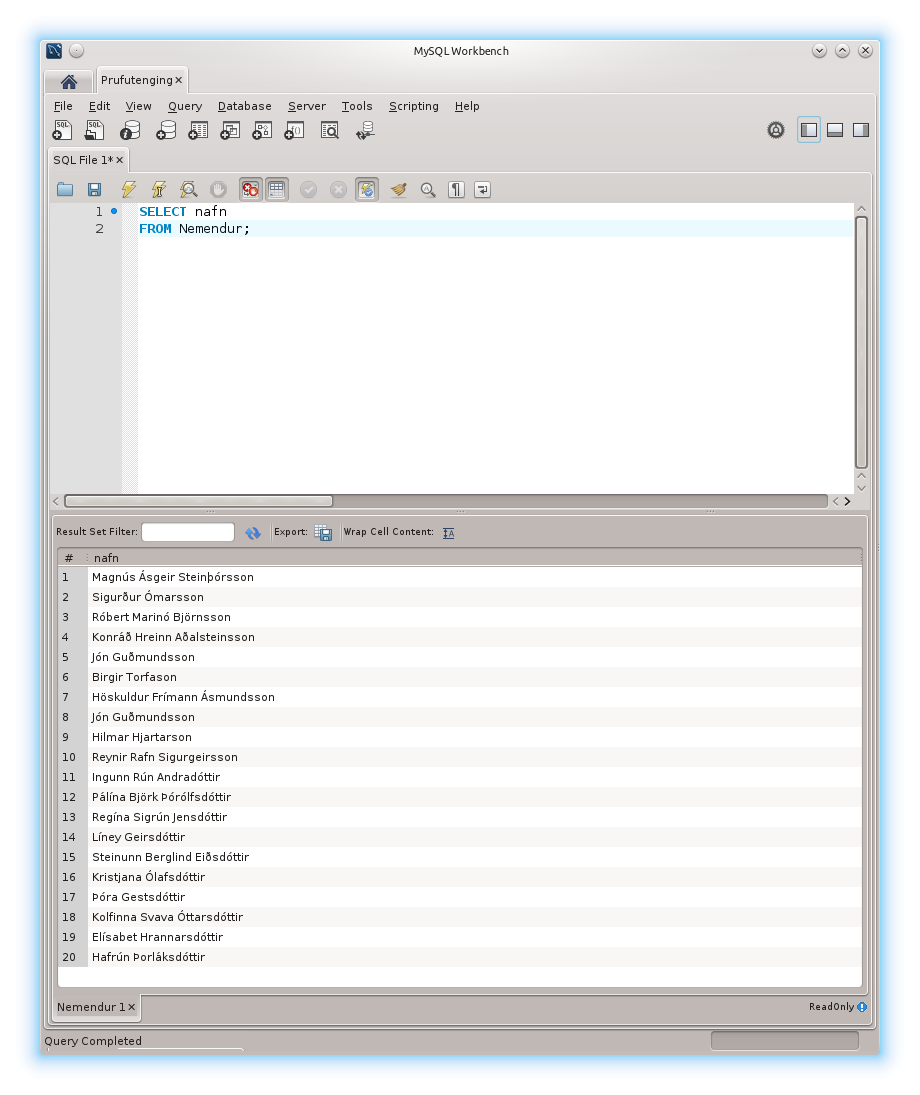
\includegraphics[width=\linewidth]{myndir/workbench-select}
\end{figure*}

\verb|SELECT| skipun getur náð í marga dálka (eða mörg atriði) í einu. Atriðin eru þá einfaldlega aðgreind með kommum. Þetta má sjá á sýnidæmi \ref{sql:k4d3-margir-dalkar}.

\begin{example}
\caption[SELECT með mörgum dálkum]{\emph{SELECT} skipun sem nær í marga dálka. }
\label{sql:k4d3-margir-dalkar}
\centering
\sql{sql/k4d3-margir-dalkar.sql}
\end{example}

\begin{table}
\centering
\caption[Niðurstaða margra dálka SELECT]{Niðurstaða skipunarinnar í sýnidæmi \ref{sql:k4d3-margir-dalkar} gæti litið út á þessa leið. Allar upplýsingarnar úr dálkunum ``nafn'' og ``kennitala'' voru valdar. Aðrir dálkar sjást ekki.}
\label{tafla:margir-dalkar-nidurstada}
\begin{tabular}{ll}
\toprule
nafn&kennitala\\
\midrule
Magnús Ásgeir Steinþórsson&090698-6489\\
Sigurður Ómarsson&251198-1369\\
Róbert Marinó Björnsson&060998-2489\\
Konráð Hreinn Aðalsteinsson&120498-8869\\
Kári Jensson&230598-2159\\
Birgir Torfason&170798-7249\\
Höskuldur Frímann Ásmundsson&020298-4139\\
Styrmir Hreinsson&210498-7889\\
Hilmar Hjartarson&020798-4599\\
Reynir Rafn Sigurgeirsson&211298-7239\\
Ingunn Rún Andradóttir&161298-1589\\
Pálína Björk Þórólfsdóttir&030798-0829\\
Regína Sigrún Jensdóttir&140798-6499\\
Líney Geirsdóttir&111098-3289\\
Steinunn Berglind Eiðsdóttir&190398-1889\\
Kristjana Ólafsdóttir&230298-4759\\
Þóra Gestsdóttir&010498-8489\\
Kolfinna Svava Óttarsdóttir&210498-5759\\
Elísabet Hrannarsdóttir&050298-3109\\
Hafrún Þorláksdóttir&250498-2849\\
\bottomrule
\end{tabular}
\end{table}

\begin{figure*}
\caption[Niðurstöður margra dálka SELECT í Workbench]{Hér sést hvernig sýnidæmi \ref{sql:k4d3-margir-dalkar} og niðurstaða \emph{SELECT} skipunarinnar sem í því er (tafla \ref{tafla:margir-dalkar-nidurstada}) getur litið út í MySQL Workbench.}
\label{mynd:workbench-nidurstada-margir-dalkar}
\centering
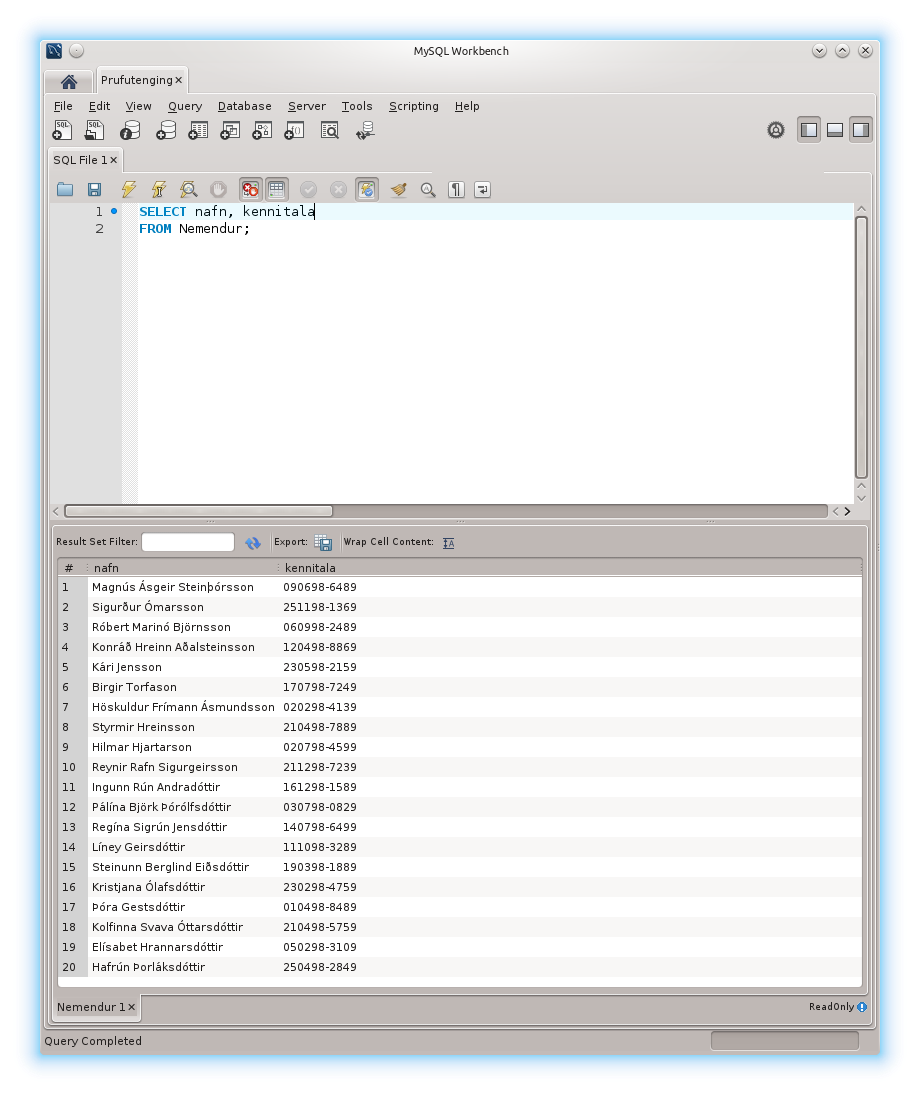
\includegraphics[width=\linewidth]{myndir/workbench-nidurstada-margir-dalkar}
\end{figure*}
\section{WHERE klausan}
Hingað til höfum við valið heila dálka með \verb|SELECT| skipunum. Það sem við viljum hins vegar oftast gera er að finna ákveðnar upplýsingar í töflunni, frekar en að fá þær allar.

Til þess að fá bara þær upplýsingar sem við viljum búum við til ``síu'' sem hleypir engum upplýsingum í gegn nema þeim sem við viljum.

Slík sía þarf að innihalda lýsingu á þeim gögnum sem hleypa á í gegn. Það er gert í klausu sem við köllum \verb|WHERE| klausu og kemur fyrir aftan \verb|FROM| klausuna. Dæmi um þetta má sjá í sýnidæmum \ref{sql:k4d4-where-numer} til \ref{mynd:workbench-nidurstada-jon}.

\begin{example}
\caption[SELECT með WHERE klausu - eftir númeri]{\emph{SELECT} skipun með \emph{WHERE} klausu sem nær í nafn nemanda (úr töflu \ref{tafla:nemendur}) þar sem ``numer'' dálkurinn er með gildið 11. Hún skilar einni línu, nafninu Ingunn Rún Andradóttir.}
\label{sql:k4d4-where-numer}
\centering
\sql{sql/k4d4-where-numer.sql}
\end{example}

\begin{example}
\caption[SELECT með WHERE klausu - eftir nafni]{\emph{SELECT} skipun með \emph{WHERE} klausu sem nær í kennitölu nemanda eftir nafni hans. Hún skilar einni línu, kennitölunni 251198-1369.}
\label{sql:k4d5-where-nafn}
\centering
\sql{sql/k4d5-where-nafn.sql}
\end{example}

\begin{example}
\caption[SELECT með WHERE klausu - endurtekin gildi]{Skilyrðið sem sett er fram í \emph{WHERE} klausu getur átt við meira en eina línu í töflunni. Þessi skipun finnur nöfn og kennitölu allra sem heita Jón Guðmundsson. Þeir reynast vera tveir, með kennitölurnar 230598-2159 og 210498-7889.}
\label{sql:k4d6-where-nafn-endurtekid}
\centering
\sql{sql/k4d6-where-nafn-endurtekid.sql}
\end{example}

\begin{figure*}[h]
\caption[Niðurstöður margra dálka SELECT í Workbench]{Hér sést sýnidæmi \ref{sql:k4d6-where-nafn-endurtekid} í MySQL Workbench.}
\label{mynd:workbench-nidurstada-jon}
\centering
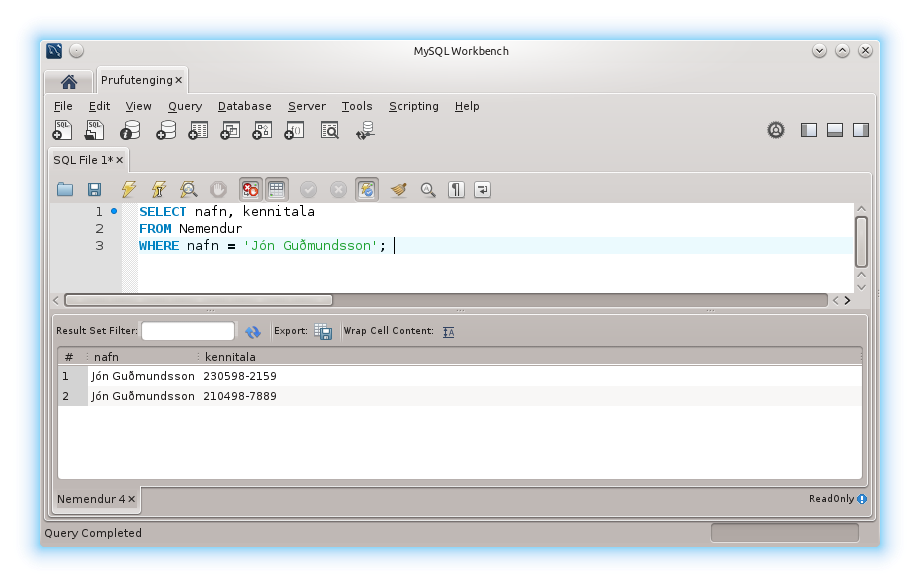
\includegraphics[width=\linewidth]{myndir/workbench-nidurstada-jon}
\end{figure*}
\subsection{Samanburðir í WHERE}
Í öllum \verb|WHERE| klausunum hér á undan er um að ræða síur sem henda öllu sem ekki uppfylla eitt, nákvæmt skilyrði. Skilyrðið í sýnidæmi \ref{sql:k4d4-where-numer}, \verb|numer = 11|, hleypir til dæmis einungis þeim nemanda sem er með nákvæmlega númerið 11 í gegn.

Skilyrðin geta þó verið margs konar. Skilyrðið \verb|numer > 11| hleypir til dæmis öllum línum í gegn þar sem gildið í ``numer'' dálkinum er stærra en 11. Yfirlit yfir mögulega samanburði má sjá á töflu \ref{tafla:samanburdir}.

\begin{table*}
\centering
\caption[Samanburðir]{Samanburðir sem nota mætti í \emph{WHERE} klausu \emph{SELECT} skipunar. Hér er \emph{numer} nafnið á dálki sem inniheldur tölur.}
\label{tafla:samanburdir}
\begin{tabular}{ll}
\toprule
Dæmi&Útskýring\\
\midrule
\emph{numer} = 5&Hleypir þeim línum í gegn þar sem gildið í \emph{numer} er nákvæmlega 5.\\
\emph{numer} > 5&Hleypir þeim línum í gegn þar sem gildið í \emph{numer} er stærra en 5.\\
\emph{numer} < 5&Hleypir þeim línum í gegn þar sem gildið í \emph{numer} er minna en 5.\\
\emph{numer} >= 5&Hleypir þeim línum í gegn þar sem gildið í \emph{numer} er 5 eða stærra.\\
\emph{numer} >= 5&Hleypir þeim línum í gegn þar sem gildið í \emph{numer} er 5 eða minna.\\
\emph{numer} != 5 eða \emph{numer} <> 5&Hleypir þeim línum í gegn þar sem gildið í \emph{numer} er ekki 5.\\
\bottomrule
\end{tabular}
\end{table*}
\subsection{LIKE og ``wildcards''}

\subsection{Mörg aðskilin skilyrði} % AND, OR, IN
\section{Helstu einindaföll}
\subsection{LENGTH}
\subsection{ROUND}
\subsection{UCASE og LCASE}
\section{GROUP BY}
\section{Helstu samsteypuföll}
\subsection{SUM og AVG}
\subsection{MIN og MAX}
\subsection{COUNT}
\section{HAVING}
\section{ORDER BY}
\subsection{LIMIT}
\section{Yfirlit}
\subsection{Uppbygging SELECT skipunarinnar}